\section{Results / Numerical Benchmarking}
\label{sec:results}

here we'll "benchmark" (aka numerically compute the cost - number of qubits and gates - of creating a lobe block-encoding) for some systems

%ideas of systems to benchmark on:
%
%- Fermi-Hubbard 
%
%- Something with just bosons
%
%- Something with fermions, antifermions, and bosons

\subsection{Pair Production/Annihilation}
\subsubsection{Hamiltonian}
In quantum field theory, particles can spontaneously be created or annihilated (hence why second quantization is useful). A particle-antiparticle pair can annihilate each other and produce a new particle, or another particle can decay and produce a particle-antiparticle pair. This can be shown in \emph{Feynman diagrams}:

\begin{figure}[h]
    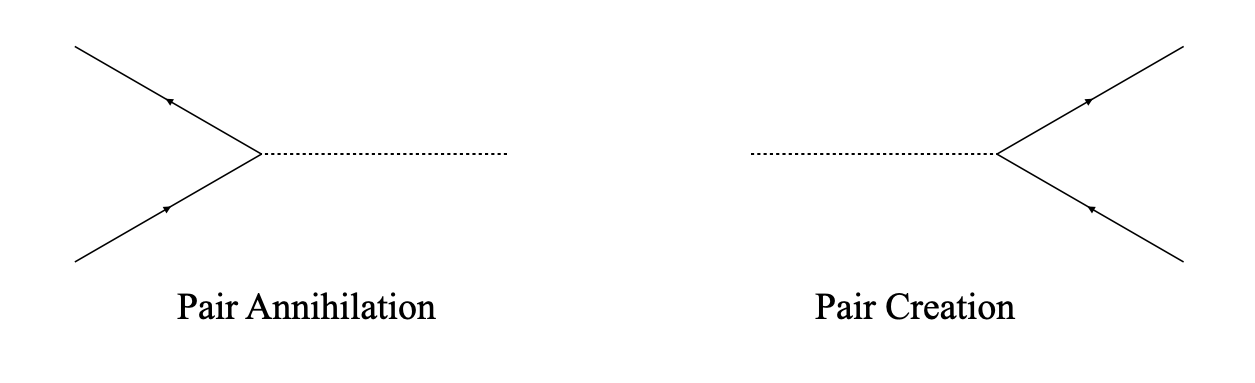
\includegraphics[width = 0.7\linewidth]{figures/creation_annihilate.png}
\end{figure}


Without going into the mathematics of this, we can contrive a toy Hamiltonian that describes this procedure:

\begin{equation}
    \label{H_pair}
    H = \sum_n^{\Lambda_{f}} b_n^\dagger b_n + \sum_n^{\Lambda_{af}} d_n^\dagger d_n + \sum_n^{\Lambda_{b}} a_n^\dagger a_n + \sum_{i,j,k}^{\Lambda_f, \Lambda_{af}, \Lambda_b} \left(b_i^\dagger d_j^\dagger a_k + b_i d_j a_k^\dagger \right).
\end{equation}

The first three terms are the kinetic energies of the individual particles ($b_n$ corresponds to a fermion, $d_n$ corresponds to an antifermion, $a_n$ corresponds to a boson). The last term describes the pair creation and pair annihilation respectively. 
Since this is a toy model, we take small mode cutoffs: $\Lambda_f = \Lambda_{af} = \Lambda_b = 2$. Additionally, it is necessary to set an occupancy cutoff for bosons. This will be set to $\Omega = 3$. The number of qubits for this problem is 17 (1 for validation, 1 for control, 1 for coefficient ancilla, 1 for normalization coefficient ancilla, 5 for the index qubits (there are 22 terms in the Hamiltonian), 8 for $\ket{\psi}$ (2 for fermions, 2 for antifermions, 2 for each of the 2 bosonic modes)).

Each term in the Hamiltonian will get its own unitary that block encodes it. The circuit loosely appears as follows:

\begin{figure}[h]
    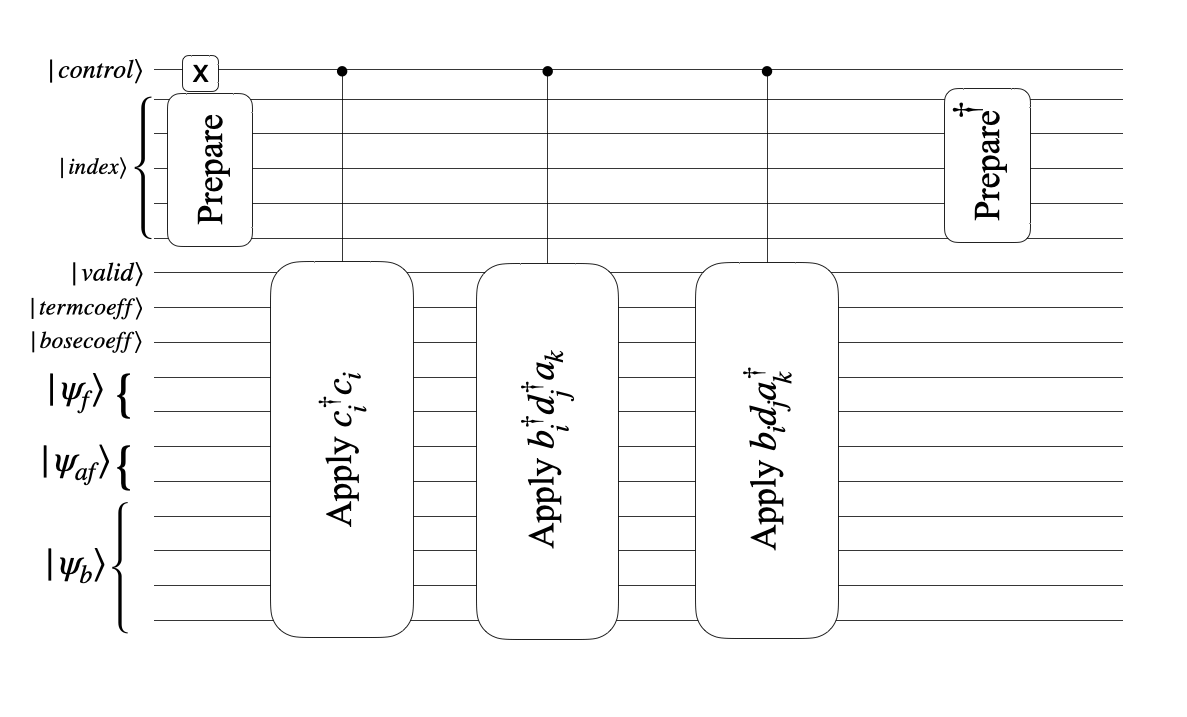
\includegraphics[width = \linewidth]{figures/H_example_LOBE_circuit.png}
\end{figure}

In what follows, we show the explicit form of the first \textit{Apply} unitary, as well as one example term from each of the following two \textit{apply} unitaries:

\begin{figure}[h]
    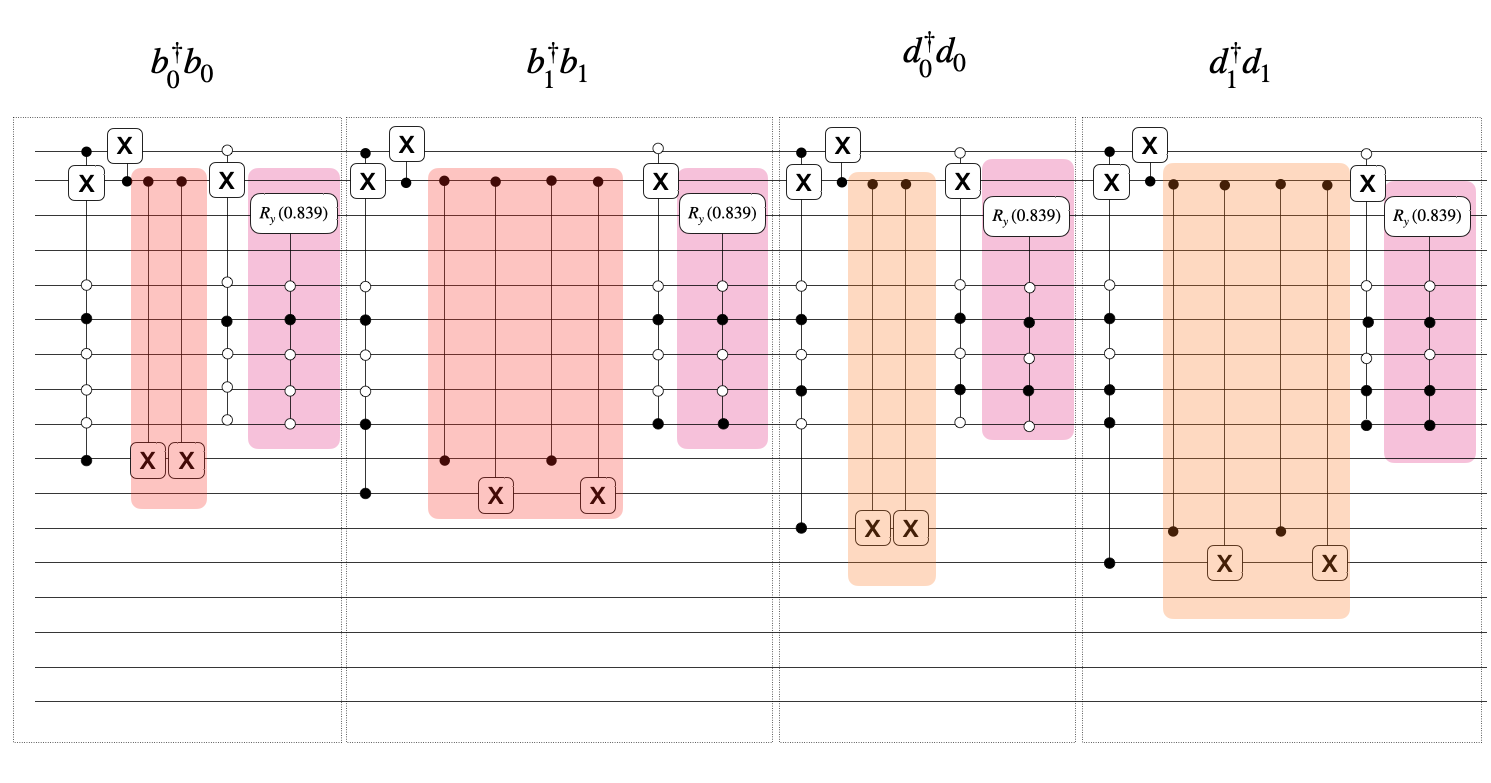
\includegraphics[width = 8cm]{figures/fermi_free.png}
    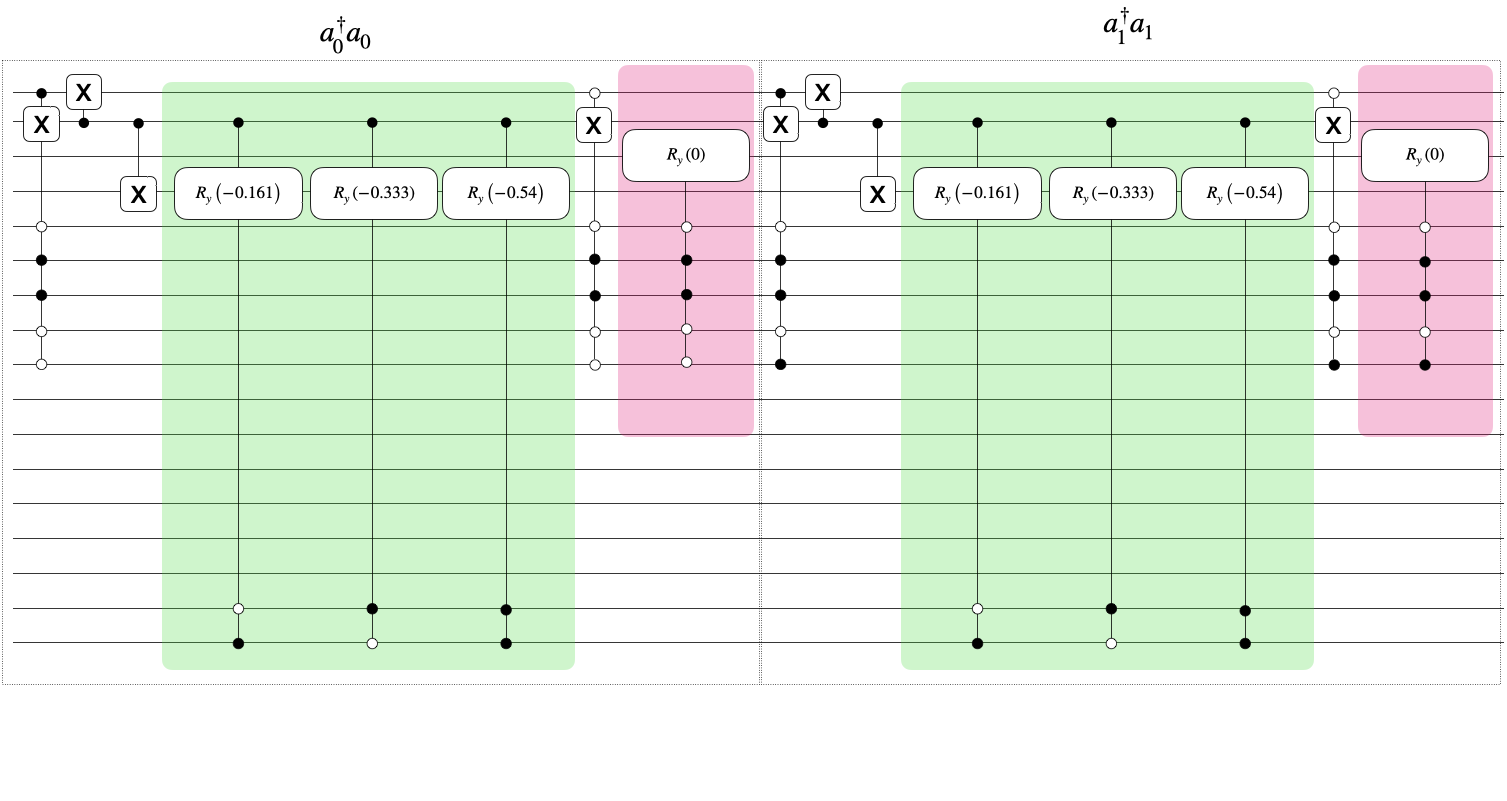
\includegraphics[width = 8cm]{figures/bose_free.png}
    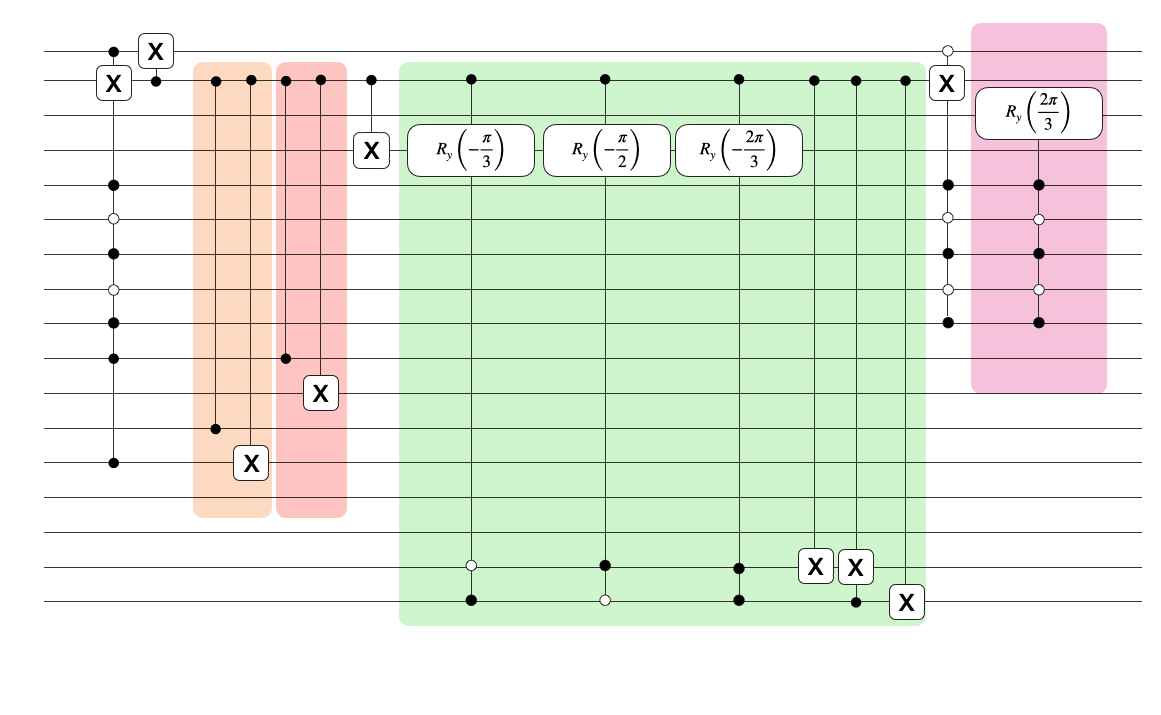
\includegraphics[width = 8cm]{figures/pair_create.png}
    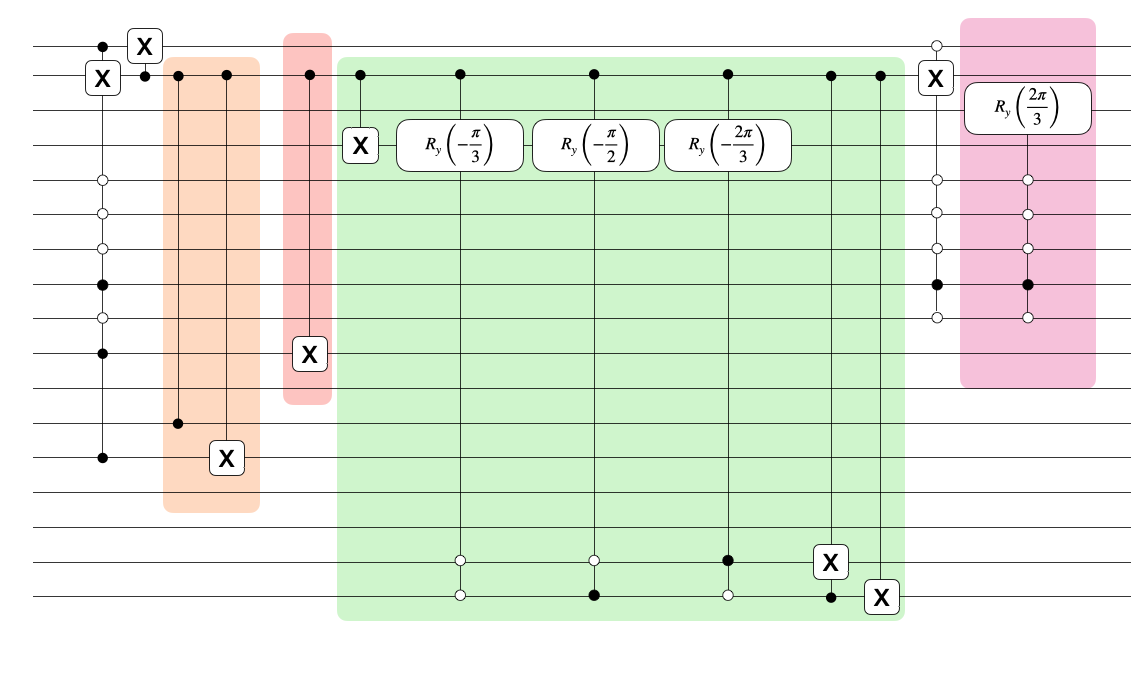
\includegraphics[width = 8cm]{figures/pair_annihilate.png}
    \caption{Applying the fermionic free Hamiltonian}
\end{figure}
